\documentclass[12pt,tikz,border=10pt]{standalone}
\usepackage{tikz}
\usetikzlibrary{scopes}
\usepackage{verbatim}
\usetikzlibrary{calc,angles,patterns,quotes,positioning,shapes}
\usetikzlibrary{patterns.meta}
\usepackage{pgfplots}
\usepackage{pgf}
\usepackage[dvipsnames]{xcolor}
\usetikzlibrary{math}
\usetikzlibrary{backgrounds}
\pgfplotsset{compat=newest}
\pgfplotsset{plot coordinates/math parser=false}



\begin{document}

\def\down{-90}
\def\ang{30}
\def\hgt{10em}
\def\lwdth{0.2em}
\def\R0{10.7em}
\def\r0{2.7em}
\def\dotr{0.1em}
\def\parcelangle{30}

\def\totalWaterLengthX{45em}
\def\totalWaterHeightZ{21em}
\def\wallWidth{1em}
\def\parcelHalfHeight{0.2*\totalWaterHeightZ}


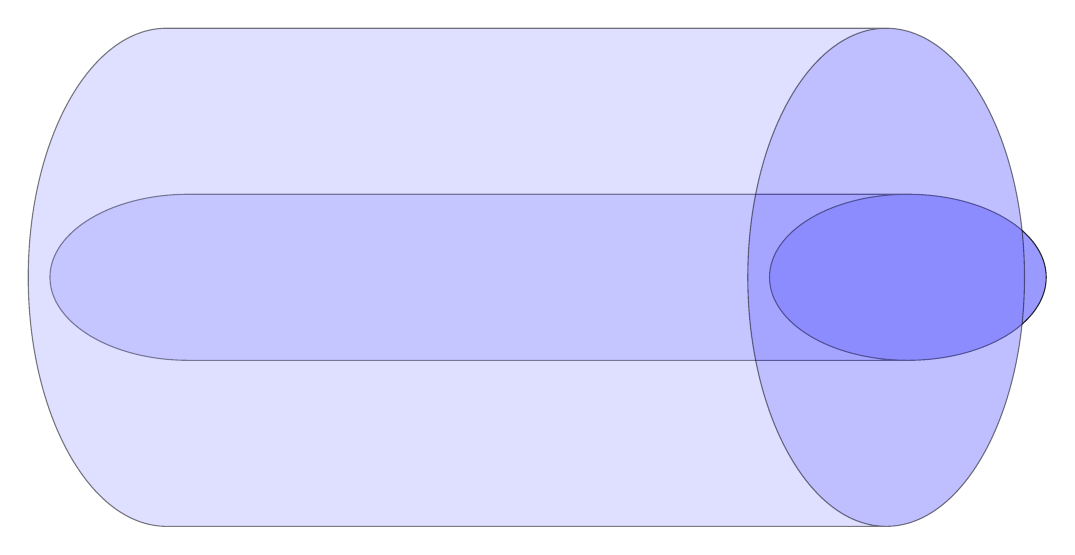
\begin{tikzpicture}[
    force/.style={>=latex,draw=blue,fill=blue,line width=\lwdth},
    axis/.style={>=latex,dashed,gray, line width=0.15em, 
                 dash pattern=on 8pt off 3pt},
    M/.style={rectangle,draw,fill=lightgray,minimum size=0.5cm,thin},
    m/.style={rectangle,draw=black,fill=lightgray,minimum size=0.3cm,thin},
    plane/.style={draw=black,fill=blue!10},
    string/.style={draw=red, thick},
    pulley/.style={thick},
    point/.style={inner sep=0, minimum width=0, text=black},
    timber-fill/.style={pattern={
        Lines[distance=8.5pt, angle=45]},
        pattern tile/.style={clip=false},
        pattern color=black
    },
    timber-fill-top/.style={
        pattern={Lines[distance=8.5pt, angle=135]}, 
        pattern tile/.style={clip=false},
        pattern color=black
    },
    scale=1.2
]


    \tikzstyle{every node}=[font=\Large];

    
    
    
    \node[cylinder, draw, shape aspect=2.5, 
          cylinder uses custom fill, cylinder end fill=blue!50, 
          minimum height=6em, minimum width=1em,
          cylinder body fill=blue!25, opacity=0.8, 
          scale=6, rotate=0]{};


    \node[cylinder, draw, shape aspect=2.5, 
          cylinder uses custom fill, cylinder end fill=blue!50, 
          minimum height=6em, minimum width=3em,
          cylinder body fill=blue!25, opacity=0.5, 
          scale=6, rotate=0]{};
 
    
\end{tikzpicture}

\end{document} 